\section{Customizable Guidance}

The customizable guidance system is a major component of our indoor navigation solution. It manages the generation and updating of QR codes for each building and also supports the backend for our mobile application. This system enables dynamic QR codes that only encode an ID, with all additional information being retrieved from a central database based on that ID. \\\\
\noindent
\textbf{The system is composed of multiple parts that interact with each other:}
 \begin{itemize} 
 	\item A front-end application for end-users, which includes two types of users: 
 	\begin{itemize} 
 		\item Building managers 
 		\item Visually impaired individuals 
 	\end{itemize} 
 	\item A backend infrastructure, which handles: \begin{itemize} 
 		\item QR code generation
 		 \item Storing necessary data in a database
 		  \item Serving API requests for the front-end applications
 	   \end{itemize}
     \end{itemize}

Each part of the system will be explained in the following subsections.

\begin{figure}[h] \centering 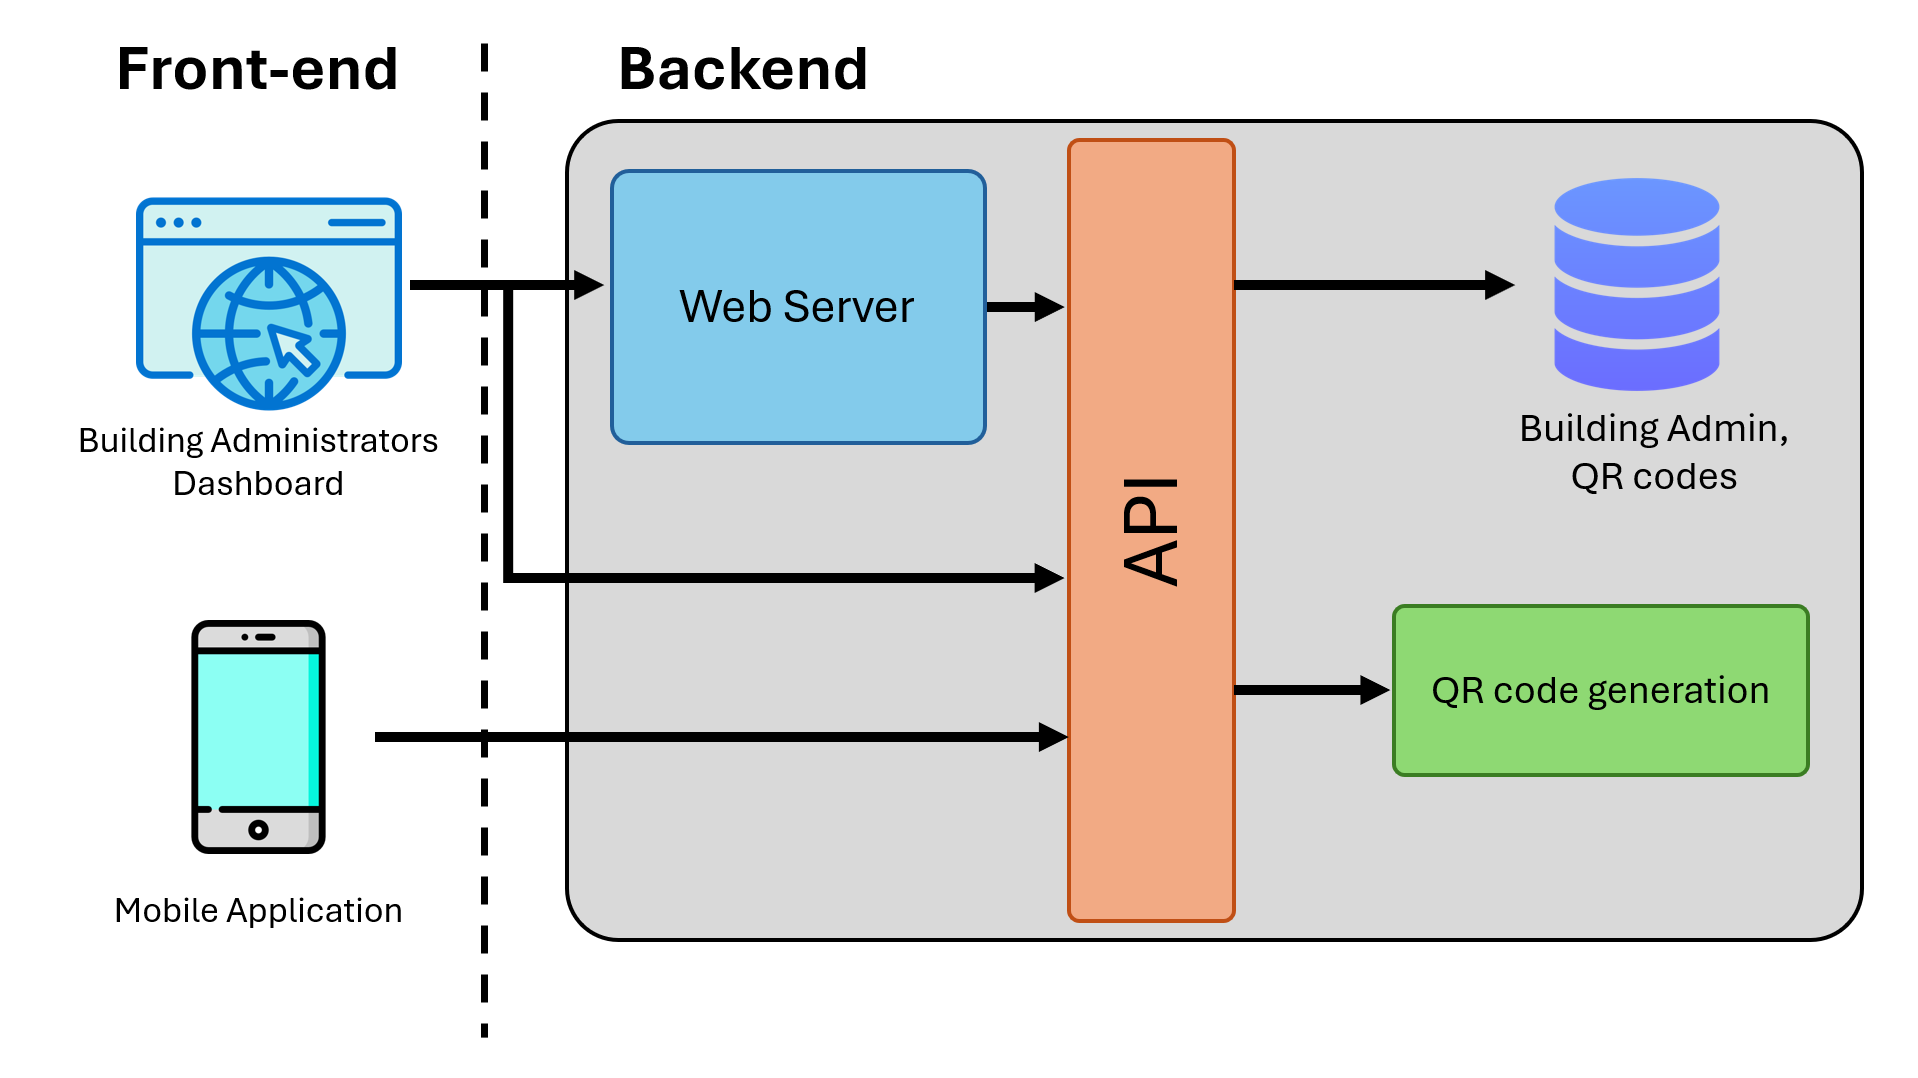
\includegraphics[width=1\textwidth]{assets/ch3/building_management_dashboard_system_overview.png} 
	\caption{System Architecture} 
	\label{fig}
\end{figure}

\subsection{Front-End Application}

The front-end consists of two interfaces: a web-based dashboard for building managers and a mobile app for visually impaired users. These interfaces provide intuitive access to the navigation system and ensure that users can easily interact with the data.

\subsubsection{Building Administrators Dashboard}

The Building Management Dashboard is a web platform where administrators can manage the navigation system for their respective buildings. This dashboard helps administrators handle the placement and updating of QR codes, each associated with navigation guidance for visually impaired users.

The dashboard consists of several key pages: \begin{itemize} \item \textbf{Sign-In/Sign-Up Page}: Allows users to create an account or log into their existing profile. \item \textbf{Profile Page}: Displays a list of buildings under the user's management. \item \textbf{Building Profile Page}: Shows details for each building, including the list of floors and related information. \item \textbf{Floor Profile Page}: Lists QR codes for each floor, with details such as QR\_ID, Section\_ID, global position (x, y), and any instructions associated with each code. \end{itemize}



This structured layout helps building managers to efficiently manage QR codes and related navigation data, ensuring that any updates are quickly reflected in the system.

\subsubsection{Visually Impaired Mobile Application}

The mobile application is designed to assist visually impaired users by guiding them through indoor spaces using the QR codes placed around the building. The app functions as a navigation tool, with the following key features:

\begin{itemize} 
	\item \textbf{Main Screen}: The initial interface of the app, allowing access to the main navigation features. 
	\item \textbf{Navigation Screen}: After scanning a QR code, the app provides real-time instructions based on the user’s current location.
 \end{itemize}

The mobile app connects to the backend infrastructure to retrieve the relevant navigation data based on the QR code ID.

\subsection{Back-End Infrastructure}

The backend serves as the core of the customizable guidance system. It manages the storage of user data, QR codes, and instructions, and ensures seamless communication between the front-end and the database. The key components of the backend include the web server, API, and database.

\subsubsection{Web Server}

The web server hosts the dashboard for building managers, allowing them to sign in, manage buildings, floors, and QR codes. It handles the presentation of data from the database to the front-end interface, ensuring that building administrators can make real-time updates.

\subsubsection{Application Programming Interface (API)}

The API acts as a bridge between the mobile app and the building management dashboard. It handles various requests such as user authentication, QR code management, and instruction updates.

The API consists of multiple endpoints, each handling specific tasks. For example, one method allows administrators to add instructions for an entire floor, which will update the associated QR codes with new navigation information. Figure \ref{fig:api_method} demonstrates this API method. Full API documentation are presented on Appendix A (to be added). 

\begin{figure}[h] \centering \includegraphics[width=0.5\textwidth]{example-image-a} \caption{API Method: Add instruction to entire floor} 
	\label{fig:api_method} 
	\end{figure}

\subsubsection{Database}

The backend uses a relational database with two main tables: one for user credentials and another for QR code data, with a foreign key relationship linking them. This design ensures scalability, easier management, and efficient querying across users and QR codes.

A visual overview of the database schema is shown in Figure \ref{fig:database_schema}.

\begin{figure}[h]
	\centering
	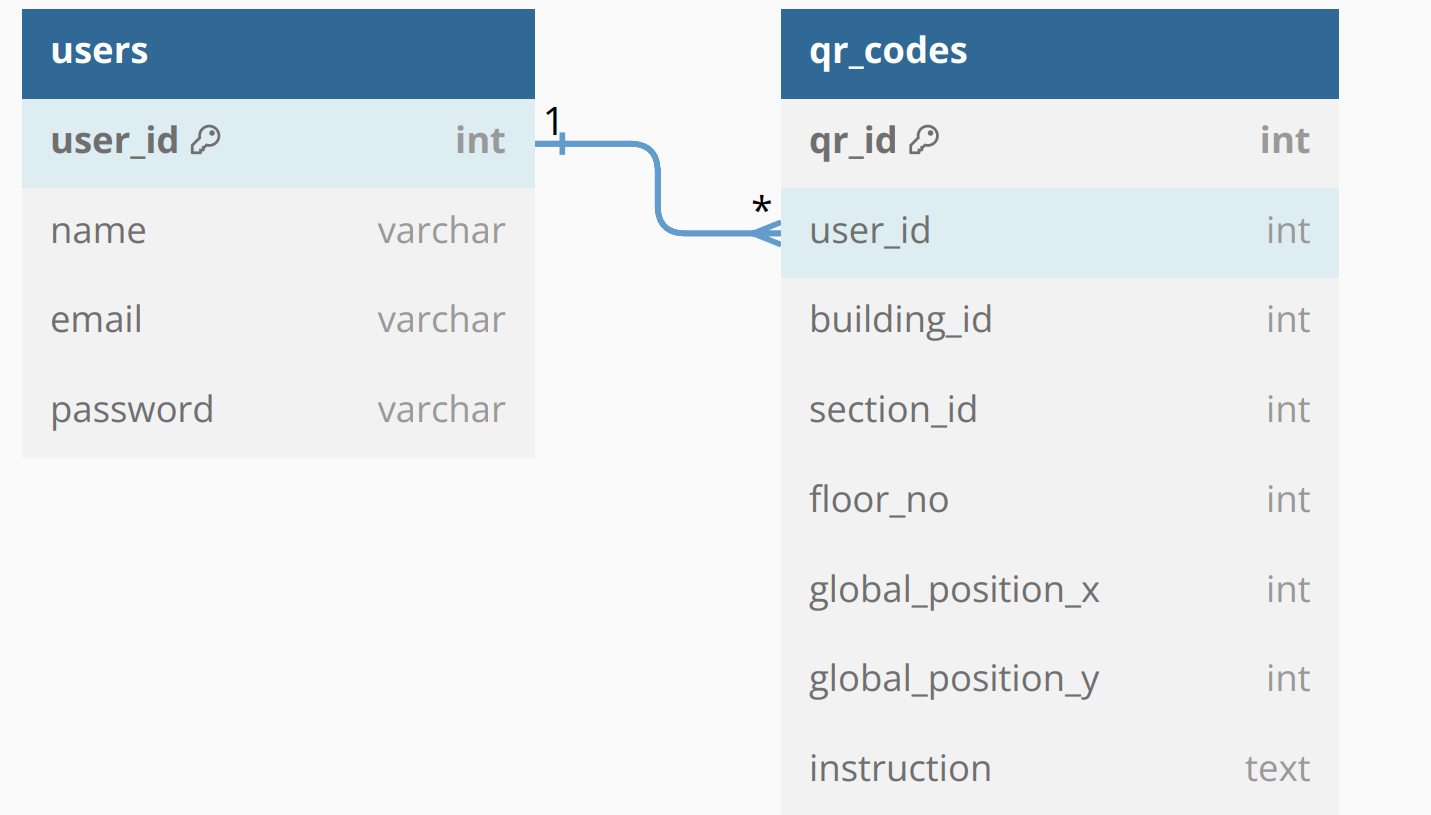
\includegraphics[width=0.9\textwidth]{assets/ch3/db_schema.png}
	\caption{Database Schema for Users and QR Codes}
	\label{fig:database_schema}
\end{figure}

\begin{itemize}
	\item \textbf{Users Table}: This table stores user credentials and uniquely identifies each user. The fields include:
	\begin{itemize}
		\item \textbf{User\_ID} (Primary Key): A unique identifier for each user.
		\item \textbf{Name}: The user's name.
		\item \textbf{Email}: The user's email address.
		\item \textbf{Password}: Encrypted password for authentication.
	\end{itemize}
	
	\item \textbf{QR Codes Table}: This table stores QR code data for each user. It includes a foreign key linking to the users table to associate QR codes with their respective users. The fields include:
	\begin{itemize}
		\item \textbf{QR\_ID} (Primary Key): A unique identifier for each QR code.
		\item \textbf{User\_ID} (Foreign Key): Links the QR code to the associated user from the users table.
		\item \textbf{Building\_ID}: Unique identifier for each building.
		\item \textbf{Floor\_No}: Indicates the floor number where the QR code is located.
		\item \textbf{Section\_ID}: Identifies the section within the floor.
		\item \textbf{Global Position X, Global Position Y}: Coordinates representing the location of the QR code.
		\item \textbf{Instruction}: Instructions linked to the QR code.
	\end{itemize}
\end{itemize}


